La notion de notation musicale exécutable est intimement lié au format de partition numérique. Deux sens peuvent être prêtés au terme de notation musicale exécutable. 
Premièrement, une partition est exécutable si elle peut contribuer à la production d'un résultat musical, ou sonore, lors de sa lecture par un ordinateur. Il existe alors une dépendance (\textit{mapping}) entre les paramètres graphiques de la partition et les paramètres de production du son. Cette dépendance permet aussi bien à une partition de piloter un synthétiseur que de transcrire graphiquement les variations dans le jeu musical de ce même synthétiseur.

Deuxièmement, l'exécutabilité d'une notation peut également provenir des actions de modification de son propre contenu (modification graphique ou sur les données envoyées) lors de sa lecture temporelle. Par exemple, un  symbole placé sur une partition peut être un déclencheur d'évènement, qui à sa lecture entraîne la modification de la partition (création, modification, suppression d'autres symboles…). Cette logique de fonctionnement est celle utilisée par INScore pour la création de partitions \textit{interactives} \cite{fober2017}.
Aussi, cette idée d'encapsulation d'intelligence programmationnelle dans un symbole est atteinte dans \textit{symbolist} grâce à l'utilisation de la librairie \textit{odot} et son système d'expressions \cite{maccallum2011}.

\subsection{La librairie odot}
\label{subsec:odotLibrary}
La librairie \textit{odot}, développée au laboratoire CNMAT de l'Université de Berkeley, offre une implémentation en langage C du format OSC augmenté de certaines possibilités. Notamment, le \og format \fg \textit{odot} multiplie les types de données pouvant être contenus dans un message OSC. Par exemple, un bundle OSC peut être stocké dans un message, rendant possible l'imbrication de bundles (comme au format JSON). 
La librairie \textit{odot} a été encapsulé en C++ afin d'être intégré à \textit{symbolist}. Comme évoqué plus haut, \textit{odot} met à disposition un langage de programmation, appelé \textit{o.expr}, qui permet d'appliquer des expressions \og à la C \fg à des bundles OSC. \textit{o.expr} permet d'ajouter des messages à un bundle OSC ou de modifier la valeur d'un message préexistant. La figure \ref{fig:applyOdotExpr} donne un exemple de bundle OSC avant et après l'application d'une expression \textit{odot}.

\begin{figure}[H]
	\centering
	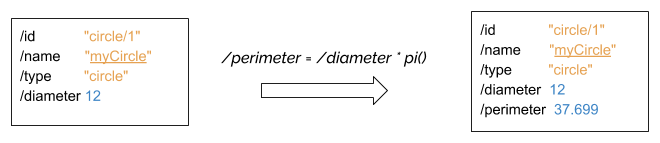
\includegraphics[keepaspectratio=true, width=\textwidth]{ModeleDeNotation/i/applyOdotExpr.png}
	\caption{Application d'une expression odot à un bundle OSC}
	\label{fig:applyOdotExpr}
	\small
	\textit{A gauche, le bundle OSC avant l'application de l'expression \emph{/perimeter = /diameter * pi()}. A droite, le bundle OSC résultant.}
\end{figure}

Le langage d'expressions \textit{odot} met à disposition de l'utilisateur un certain nombre de primitives: des fonctions pour le calcul mathématique (\texttt{pi()}, \texttt{e()}, \texttt{sum()}, \texttt{product()}...), des fonctions pour la recherche et le listing d'adresses et de valeurs de messages OSC (\texttt{getadresses()}, \texttt{getvalues()}...), mais aussi la possibilité de définir des lambda fonctions et des fonctions de mapping (\texttt{lambda()}, \texttt{map()}...).

Une des contributions de ce stage a été de rendre possible l'application d'expressions \textit{odot} à un symbole (qui est sous-jacemment un bundle OSC) dans une partition \textit{symbolist}. L'application d'une expression \textit{odot} à un symbole passe par l'inspecteur de l'interface \textit{symbolist}, comme montré en figure \ref{fig:evaluateBundle}.

\begin{figure}[H]
	\centering
	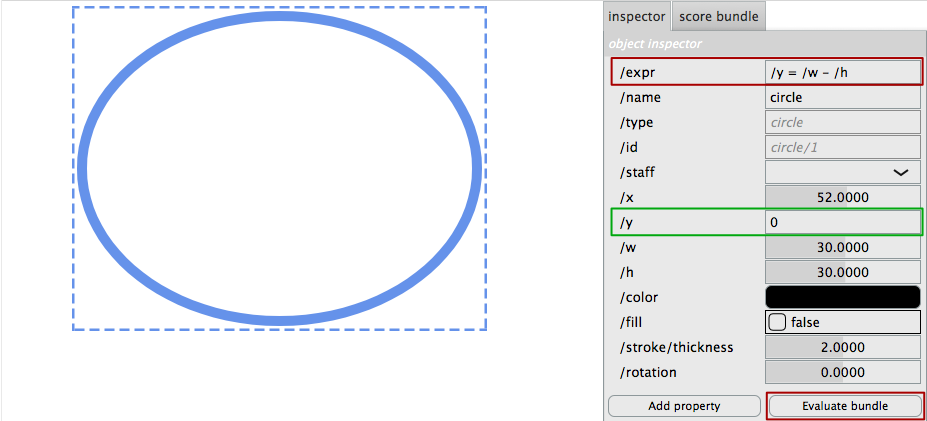
\includegraphics[keepaspectratio=true, width=\textwidth]{ModeleDeNotation/i/evaluateBundle.png}
	\caption{Evaluation d'un bundle via l'interface de symbolist}
	\label{fig:evaluateBundle}
	\small
	\textit{En \textcolor{red}{rouge}, l'expression \emph{odot} à évaluer pour le symbole courant (l'ovale bleu sélectionné dans la fenêtre de gauche), et le bouton servant à lancer l'évaluation. En vert, le résultat de l'application de l'expression \emph{odot} au symbole courant (modification de la valeur du message \texttt{/y}).}
\end{figure}

Par convention, l'expression \textit{odot} à appliquer à un symbole est contenue dans le message OSC d'adresse \texttt{/expr}.
Aussi, lors de la lecture d'une partition \textit{symbolist}, chaque symbole envoyé en sortie est évalué, c'est à dire l'expression \textit{odot} contenue dans \texttt{/expr} -  sous réserve de son existence - est appliquée au symbole.
De cette manière, un nombre illimité de nouvelles informations peuvent être générées lors de la lecture d'une partition \textit{symbolist}.

\subsection{La partition comme pilote des paramètres du son} 
\label{subsec:partitionPiloteSon}
Une partition peut-être vue comme une suite d'instructions (d'évènements) pour exécuter une pièce musicale \cite{bosseur2005}. Contrairement aux interactions traditionnelles où la partition est décodée par l'interprète humain pour produire de la musique, dans un environnement numérique, la partition contrôle un ou plusieurs processus informatiques (qui deviennent à leur tour des interprètes) dans le but de produire un résultat musical (ou multimédia).
Dans \textit{symbolist}, chaque symbole de la partition est décrit par un bundle OSC (voir section \ref{sec:geneseSymbolist}), qui liste, dans un format standardisé (couples adresse-valeur), les attributs du symbole associé.
Le format OSC étant standard en informatique musicale, \textit{symbolist} en tire avantage pour pouvoir communiquer des informations contenues dans une partition à d'autres processus informatiques (application, objets, composants logiciels…), dans le but de contrôler leurs paramètres d'entrées.
Alors, la question suivante se pose: comment lier, dans un paradigme de communication OSC, les attributs d'un symbole aux paramètres d'entrée d'un processus informatique?

Une exemple simple peut être pris pour illustré le principe de connexion entre attributs de symbole et paramètres de processus. La figure \ref{fig:linkingParameters} présente un exemple de partition créée avec \textit{symbolist} qui a pour but de contrôler la hauteur du son (en Hertz) produit par un synthétiseur.

\begin{figure}[H]
	\centering
	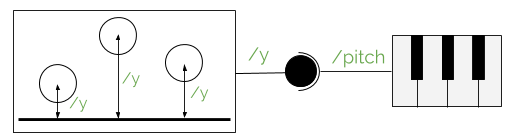
\includegraphics[keepaspectratio=true, width=\textwidth]{ModeleDeNotation/i/linkingParameters.png}
	\caption{Liaison de paramètres entre une partition et un synthétiseur}
	\label{fig:linkingParameters}
	\small
	\textit{ A gauche, une partition \textit{symbolist} constitué d'un trait horizontal et d'une suite de cercles placés plus ou moins haut selon l'axe vertical. A droite, un synthétiseur, pouvant représenté un objet (au sens instance de classe), une application, ou une machine indépendante. }
\end{figure}

Dans la figure \ref{fig:linkingParameters}, le formalisme graphique utilisé pour exprimer la connexion entre les paramètres de sortie de la partition et les paramètres d'entrée du synthétiseur est celui défini par UML 2.5.1 pour modéliser les architectures de composants \cite{omg2017}. En effet, il est pratique de considérer la partition et le synthétiseur comme deux composants logiciels pour étudier la connexion de leurs paramètres. Ici, le cercle noir attaché à la partition modélise un paramètre de sortie (\textit{interface fournie}, le message OSC \texttt{/y}), et l'arc de cercle attaché au synthétiseur représente un paramètre d'entrée (\textit{interface requise}, le message OSC \texttt{/pitch}).
Dans notre exemple, le synthétiseur a besoin de l'information \texttt{/pitch}, qui représente la hauteur du son à produire en Hertz, pour pouvoir fonctionner.
De fait, connecter le paramètre \texttt{/pitch} du synthétiseur au message \texttt{/y} envoyé par la partition lie les deux valeurs selon l'expression: $/pitch = f(/y(t))$
Soit, la hauteur du son produit par le synthétiseur est une fonction de la hauteur des cercles sur l'axe vertical évoluant au fil du temps. Cette connexion peut être effectuée de deux manières: 
\begin{enumerate}[label={(\arabic*)}]
	\item \textbf{Manuellement}: l'utilisateur devra alors connaître les paramètres d'entrée du synthétiseur et envoyé les messages correspondant en sortie lors de la lecture de la partition. Dans notre exemple, l'utilisateur devra explicitement créé un message \texttt{/pitch} pour chaque cercle de la partition et l'envoyer au synthétiseur.
	\item \textbf{(Semi-)Automatiquement}: Un protocole de communication peut être mis en place pour la connexion de \textit{symbolist} et du synthétiseur; le protocole mettra en relation les messages exposés par la partition \textit{symbolist} et les messages pouvant être reçus par le synthétiseur. Aussi, l'utilisateur devra s'assurer que les paramètres sont correctement liés, d'où le caractère semi-automatique de cette procédure. 
\end{enumerate}
%
Dans les deux cas, la fonction $f$ qui permettra, pour reprendre l'exemple, de lier la valeur de \texttt{/pitch} à \texttt{/y(t)} pourra être précisée en tirant profit des expressions \textit{odot} (voir section \ref{subsec:odotLibrary}).
Aussi, le protocole de communication devra s'assurer qu'une partition \textit{symbolist} est bien \textit{composable} avec le processus qu'elle veut contrôler. Entre autres, les interfaces exposées par l'un et l'autre doivent être compatibles \cite{chen2007}. Un des critères de la compatibilité peut simplement être la nécessité de mise en relation de paramètre du même type. Dans notre exemple, si \textit{/pitch} est de type \textit{float} et la valeur retournée par $f(/y(t))$ est une chaîne de caractères, alors la partition n'est pas composable avec le synthétiseur.

Pour réaliser cette fonctionnalité de connexion entre partition et processus de production sonore, deux technologies provenant du monde de l'informatique musicale possèdent un intérêt. La première technologie est le framework \textit{jamoma} qui permet l'encapsulation de patches Max\footnote{Pour rappel, un patch Max est une composition d'objets du langage de programmation visuelle Max. Les objets d'un patch Max sont reliés entre eux par des cordes, permettant leur communication par envoi de messages.} dans un module. Un module \textit{jamoma} déclare ses interfaces d'entrée et de sortie sous forme de liste de messages OSC, comme montré en figure \ref{fig:jamomaModule}.
\begin{figure}[H]
	\centering
	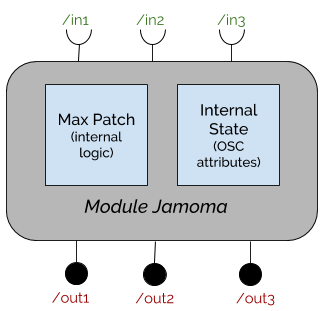
\includegraphics[keepaspectratio=true, width=0.5\textwidth]{ModeleDeNotation/i/jamomaModule.png}
	\caption{Structure d'un module jamoma}
	\label{fig:jamomaModule}
	\small
	\textit{ En haut, les connexions arc de cercle représentent l'interface d'entrée du module. En bas, les connexions en cercle rempli représentent l'interface de sortie du module.}
\end{figure}
Un module \textit{jamoma} maintient un état interne (\textit{internal state} sur la figure \ref{fig:jamomaModule}) reflétant la valeur courante des attributs exposés en entrée et en sortie du module.
La connexion entre les entrées et sorties du module et le patch Max encapsulé est définie à la création du module.
L'utilisation de modules \textit{jamoma} assure une communication basée sur l'envoi de messages au format OSC, ainsi qu'une exposition explicite des messages pouvant être envoyés et reçus par un module. 

La deuxième technologie digne d'intérêt est le protocole \textit{Minuit} qui décrit un système de requêtes entre processus utilisant le format OSC comme structure interne de données \cite{minuit2010}. \textit{Minuit} définit trois types de messages pouvant être envoyés: \texttt{get} permettant de lire la valeur d'un message OSC, \texttt{set} permettant d'écrire la valeur d'un message OSC, et \textit{listen} permettant de définir un écouteur sur une valeur de message OSC. Pour reprendre l'exemple cité plus haut, le protocole \textit{Minuit} permettrait à une partition \textit{symbolist} d'écrire ou de lire la valeur de l'attribut \textit{/pitch} du synthétiseur, ou bien permettrait au synthétiseur d'être tenu au courant de la valeur courante de \texttt{/y(t)}.

